% Options for packages loaded elsewhere
\PassOptionsToPackage{unicode}{hyperref}
\PassOptionsToPackage{hyphens}{url}
\PassOptionsToPackage{dvipsnames,svgnames,x11names}{xcolor}
%
\documentclass[
]{article}

\usepackage{amsmath,amssymb}
\usepackage{iftex}
\ifPDFTeX
  \usepackage[T1]{fontenc}
  \usepackage[utf8]{inputenc}
  \usepackage{textcomp} % provide euro and other symbols
\else % if luatex or xetex
  \usepackage{unicode-math}
  \defaultfontfeatures{Scale=MatchLowercase}
  \defaultfontfeatures[\rmfamily]{Ligatures=TeX,Scale=1}
\fi
\usepackage{lmodern}
\ifPDFTeX\else  
    % xetex/luatex font selection
\fi
% Use upquote if available, for straight quotes in verbatim environments
\IfFileExists{upquote.sty}{\usepackage{upquote}}{}
\IfFileExists{microtype.sty}{% use microtype if available
  \usepackage[]{microtype}
  \UseMicrotypeSet[protrusion]{basicmath} % disable protrusion for tt fonts
}{}
\makeatletter
\@ifundefined{KOMAClassName}{% if non-KOMA class
  \IfFileExists{parskip.sty}{%
    \usepackage{parskip}
  }{% else
    \setlength{\parindent}{0pt}
    \setlength{\parskip}{6pt plus 2pt minus 1pt}}
}{% if KOMA class
  \KOMAoptions{parskip=half}}
\makeatother
\usepackage{xcolor}
\setlength{\emergencystretch}{3em} % prevent overfull lines
\setcounter{secnumdepth}{5}
% Make \paragraph and \subparagraph free-standing
\ifx\paragraph\undefined\else
  \let\oldparagraph\paragraph
  \renewcommand{\paragraph}[1]{\oldparagraph{#1}\mbox{}}
\fi
\ifx\subparagraph\undefined\else
  \let\oldsubparagraph\subparagraph
  \renewcommand{\subparagraph}[1]{\oldsubparagraph{#1}\mbox{}}
\fi


\providecommand{\tightlist}{%
  \setlength{\itemsep}{0pt}\setlength{\parskip}{0pt}}\usepackage{longtable,booktabs,array}
\usepackage{calc} % for calculating minipage widths
% Correct order of tables after \paragraph or \subparagraph
\usepackage{etoolbox}
\makeatletter
\patchcmd\longtable{\par}{\if@noskipsec\mbox{}\fi\par}{}{}
\makeatother
% Allow footnotes in longtable head/foot
\IfFileExists{footnotehyper.sty}{\usepackage{footnotehyper}}{\usepackage{footnote}}
\makesavenoteenv{longtable}
\usepackage{graphicx}
\makeatletter
\def\maxwidth{\ifdim\Gin@nat@width>\linewidth\linewidth\else\Gin@nat@width\fi}
\def\maxheight{\ifdim\Gin@nat@height>\textheight\textheight\else\Gin@nat@height\fi}
\makeatother
% Scale images if necessary, so that they will not overflow the page
% margins by default, and it is still possible to overwrite the defaults
% using explicit options in \includegraphics[width, height, ...]{}
\setkeys{Gin}{width=\maxwidth,height=\maxheight,keepaspectratio}
% Set default figure placement to htbp
\makeatletter
\def\fps@figure{htbp}
\makeatother

\usepackage[noblocks]{authblk}
\renewcommand*{\Authsep}{, }
\renewcommand*{\Authand}{, }
\renewcommand*{\Authands}{, }
\renewcommand\Affilfont{\small}
\makeatletter
\makeatother
\makeatletter
\makeatother
\makeatletter
\@ifpackageloaded{caption}{}{\usepackage{caption}}
\AtBeginDocument{%
\ifdefined\contentsname
  \renewcommand*\contentsname{Table of contents}
\else
  \newcommand\contentsname{Table of contents}
\fi
\ifdefined\listfigurename
  \renewcommand*\listfigurename{List of Figures}
\else
  \newcommand\listfigurename{List of Figures}
\fi
\ifdefined\listtablename
  \renewcommand*\listtablename{List of Tables}
\else
  \newcommand\listtablename{List of Tables}
\fi
\ifdefined\figurename
  \renewcommand*\figurename{Figure}
\else
  \newcommand\figurename{Figure}
\fi
\ifdefined\tablename
  \renewcommand*\tablename{Table}
\else
  \newcommand\tablename{Table}
\fi
}
\@ifpackageloaded{float}{}{\usepackage{float}}
\floatstyle{ruled}
\@ifundefined{c@chapter}{\newfloat{codelisting}{h}{lop}}{\newfloat{codelisting}{h}{lop}[chapter]}
\floatname{codelisting}{Listing}
\newcommand*\listoflistings{\listof{codelisting}{List of Listings}}
\makeatother
\makeatletter
\@ifpackageloaded{caption}{}{\usepackage{caption}}
\@ifpackageloaded{subcaption}{}{\usepackage{subcaption}}
\makeatother
\makeatletter
\@ifpackageloaded{tcolorbox}{}{\usepackage[skins,breakable]{tcolorbox}}
\makeatother
\makeatletter
\@ifundefined{shadecolor}{\definecolor{shadecolor}{rgb}{.97, .97, .97}}
\makeatother
\makeatletter
\makeatother
\makeatletter
\makeatother
\ifLuaTeX
  \usepackage{selnolig}  % disable illegal ligatures
\fi
\IfFileExists{bookmark.sty}{\usepackage{bookmark}}{\usepackage{hyperref}}
\IfFileExists{xurl.sty}{\usepackage{xurl}}{} % add URL line breaks if available
\urlstyle{same} % disable monospaced font for URLs
\hypersetup{
  pdfauthor={Paweł Wiczling*},
  colorlinks=true,
  linkcolor={blue},
  filecolor={Maroon},
  citecolor={Blue},
  urlcolor={Blue},
  pdfcreator={LaTeX via pandoc}}

\title{Supporting Information for:\\
Bayesian Multilevel Modeling of Retention Data Informed by Structural
Similarity of Analytes}


  \author{Paweł Wiczling*}
            \affil{%
                  Department of Biopharmaceutics and Pharmacodynamics,
                  Medical University of Gdańsk, Gen.~J. Hallera 107,
                  80-416 Gdańsk, Poland
              }
      
\date{2025-07-18}
\begin{document}
\maketitle
\ifdefined\Shaded\renewenvironment{Shaded}{\begin{tcolorbox}[boxrule=0pt, sharp corners, breakable, enhanced, interior hidden, borderline west={3pt}{0pt}{shadecolor}, frame hidden]}{\end{tcolorbox}}\fi

\renewcommand*\contentsname{Table of contents}
{
\hypersetup{linkcolor=}
\setcounter{tocdepth}{3}
\tableofcontents
}
\newpage{}

\hypertarget{table-s1.-summary-of-the-mcmc-simulations-of-the-marginal-posterior-distributions-of-population-level-model-parameters.}{%
\section{Table S1. Summary of the MCMC simulations of the marginal
posterior distributions of population-level model
parameters.}\label{table-s1.-summary-of-the-mcmc-simulations-of-the-marginal-posterior-distributions-of-population-level-model-parameters.}}

Mean denotes sample mean, MCSE denotes Monte Carlo Standard Error,
StdDev denotes sample standard deviation, 5\%, 50\%, 95\% denote
corresponding quantiles, N\_Eff denotes effective sample size, R\_Hat
denotes a measure of chain equilibrium must be within 0.05 of 1.0.

\begin{verbatim}
  variable  mean median   sd  mad    q5   q95 rhat ess_bulk ess_tail
 logkwHat   3.05   3.05 0.19 0.19  2.74  3.36 1.00     2926     3497
 S1Hat      3.67   3.67 0.16 0.16  3.40  3.94 1.00     2598     3029
 dlogkwHat -0.35  -0.35 0.12 0.12 -0.55 -0.15 1.00     4163     3537
 dS1Hat     0.30   0.30 0.09 0.09  0.16  0.45 1.00     3403     3506
 beta[1]    0.86   0.86 0.05 0.06  0.77  0.95 1.00     3235     3620
 beta[2]    0.62   0.62 0.05 0.05  0.54  0.70 1.00     3131     3035
 S2Hat      2.90   2.90 0.03 0.03  2.85  2.95 1.02      430      935
 omega[1]   1.41   1.41 0.04 0.04  1.35  1.47 1.00     2650     2471
 omega[2]   1.13   1.13 0.03 0.03  1.08  1.18 1.00     2317     3017
 rho[1,2]   0.88   0.88 0.01 0.01  0.87  0.90 1.00     1933     2928
 sigma      0.05   0.05 0.00 0.00  0.05  0.05 1.00     1880     2927
 alpha      0.71   0.71 0.04 0.04  0.64  0.77 1.00     5245     3475
 sdpi[1]    0.15   0.14 0.02 0.02  0.11  0.18 1.01      655     1162
 sdpi[2]    0.13   0.13 0.02 0.02  0.10  0.17 1.01      641     1372
 sdpi[3]    0.34   0.33 0.06 0.06  0.23  0.44 1.00     2816     3270
 sdpi[4]    0.19   0.18 0.07 0.07  0.08  0.30 1.01      939      779
\end{verbatim}

\newpage{}

\hypertarget{figure-s1.-raw-data}{%
\section{Figure S1. Raw data}\label{figure-s1.-raw-data}}

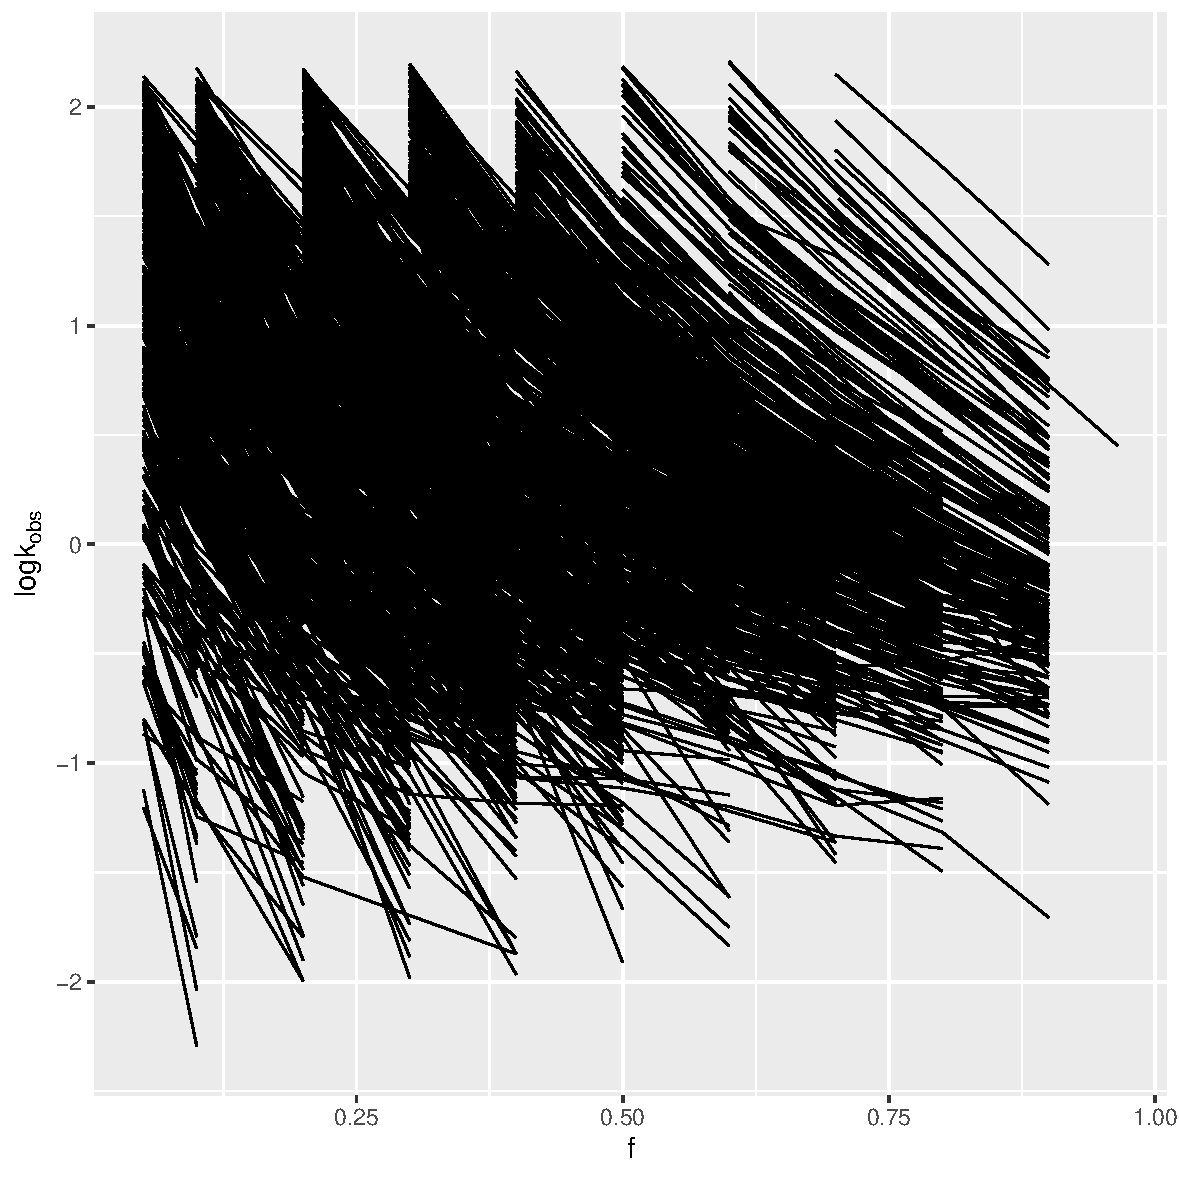
\includegraphics{../deliv/figures/manuscript/supplement/raw-data.pdf}

\newpage{}

\hypertarget{figure-s2.-functional-group-effects}{%
\section{Figure S2. Functional group
effects}\label{figure-s2.-functional-group-effects}}

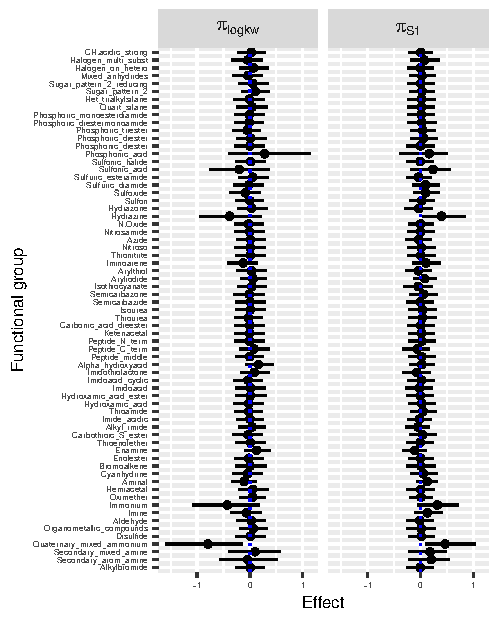
\includegraphics{../deliv/figures/manuscript/supplement/parameter-estimates-fg2.pdf}

\newpage{}

\hypertarget{figure-s3.-individual-parameters}{%
\section{Figure S3. Individual
parameters}\label{figure-s3.-individual-parameters}}

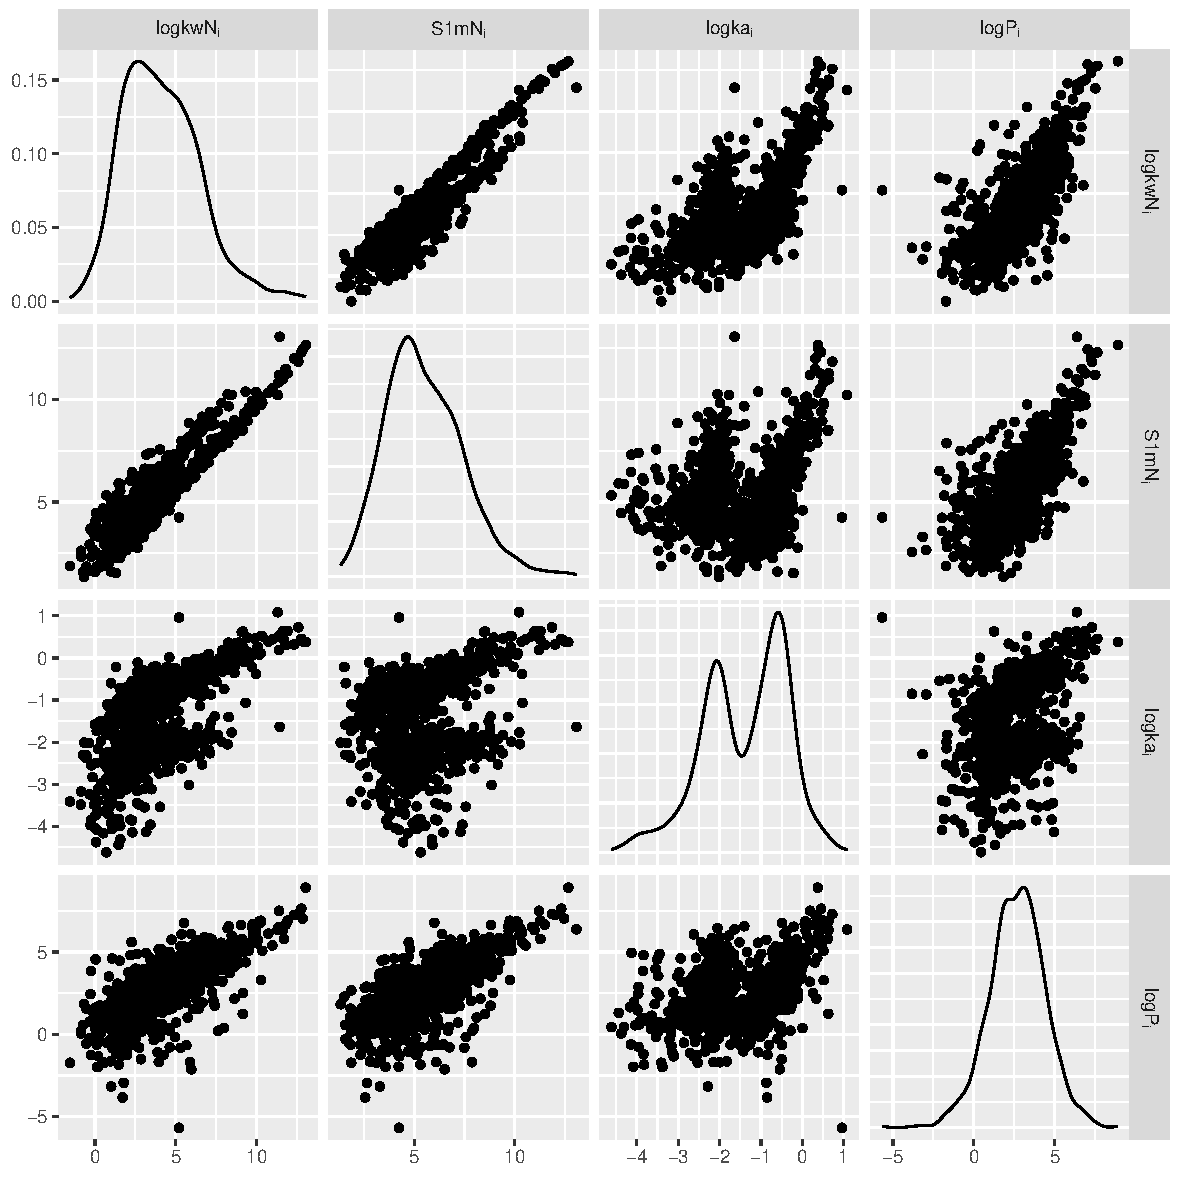
\includegraphics{../deliv/figures/manuscript/supplement/iparam.pdf}

\newpage{}

\hypertarget{figure-s4.-individual-parameters.-eta-plots}{%
\section{Figure S4. Individual parameters. Eta
plots}\label{figure-s4.-individual-parameters.-eta-plots}}

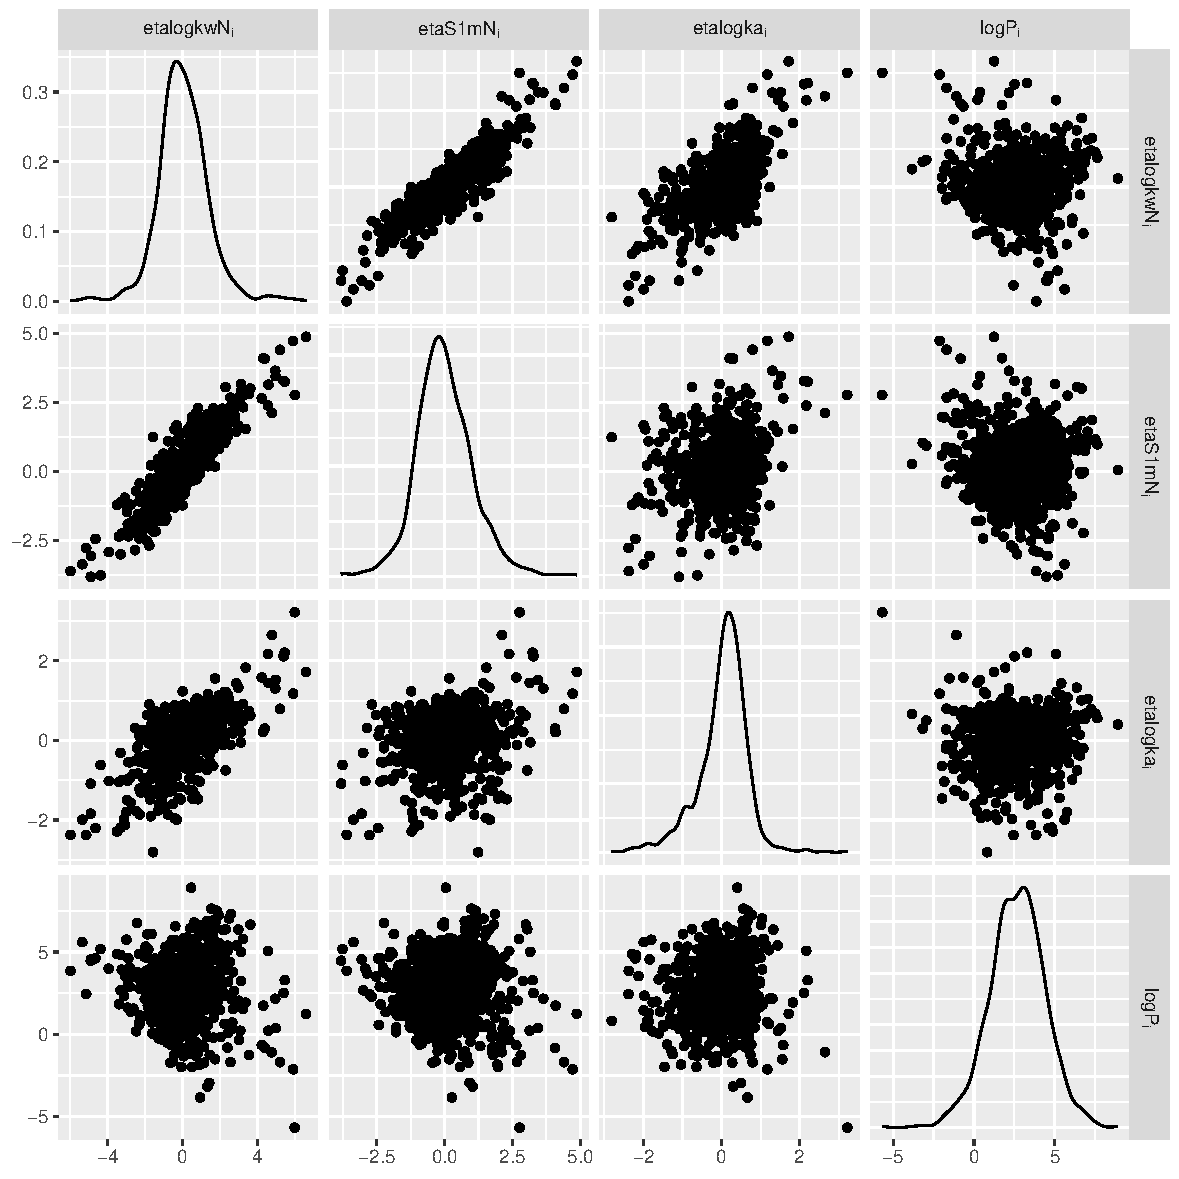
\includegraphics{../deliv/figures/manuscript/supplement/eta.pdf}

\newpage{}

\hypertarget{licenses}{%
\section*{Licenses}\label{licenses}}
\addcontentsline{toc}{section}{Licenses}

\begin{itemize}
\tightlist
\item
  Code \& copy; 2023, Paweł Wiczling, licensed under BSD-3.
\item
  Text \& copy; 2023, Paweł Wiczling, licensed under CC-BY-NC 4.0.
\end{itemize}

\hypertarget{original-computing-environment}{%
\section*{Original Computing
Environment}\label{original-computing-environment}}
\addcontentsline{toc}{section}{Original Computing Environment}

\begin{verbatim}
R version 4.3.1 (2023-06-16 ucrt)
Platform: x86_64-w64-mingw32/x64 (64-bit)
Running under: Windows 10 x64 (build 19045)

Matrix products: default


locale:
[1] LC_COLLATE=Polish_Poland.utf8  LC_CTYPE=Polish_Poland.utf8   
[3] LC_MONETARY=Polish_Poland.utf8 LC_NUMERIC=C                  
[5] LC_TIME=Polish_Poland.utf8    

time zone: Europe/Warsaw
tzcode source: internal

attached base packages:
[1] stats     graphics  grDevices utils     datasets  methods   base     

other attached packages:
[1] cmdstanr_0.8.0.9000 kableExtra_1.4.0    dplyr_1.1.4        

loaded via a namespace (and not attached):
 [1] jsonlite_1.8.8       compiler_4.3.1       tidyselect_1.2.1    
 [4] xml2_1.3.6           stringr_1.5.1        systemfonts_1.1.0   
 [7] scales_1.3.0         textshaping_0.4.0    yaml_2.3.8          
[10] fastmap_1.2.0        R6_2.5.1             generics_0.1.3      
[13] distributional_0.4.0 knitr_1.46           backports_1.5.0     
[16] checkmate_2.3.1      tibble_3.2.1         munsell_0.5.1       
[19] svglite_2.1.3        pillar_1.9.0         posterior_1.6.0     
[22] rlang_1.1.3          utf8_1.2.4           stringi_1.8.4       
[25] xfun_0.44            viridisLite_0.4.2    cli_3.6.2           
[28] withr_3.0.2          magrittr_2.0.3       ps_1.7.6            
[31] processx_3.8.4       digest_0.6.35        rstudioapi_0.16.0   
[34] lifecycle_1.0.4      vctrs_0.6.5          data.table_1.15.4   
[37] tensorA_0.36.2.1     evaluate_1.0.3       glue_1.7.0          
[40] codetools_0.2-19     ragg_1.3.2           abind_1.4-8         
[43] fansi_1.0.6          colorspace_2.1-0     rmarkdown_2.27      
[46] matrixStats_1.3.0    tools_4.3.1          pkgconfig_2.0.3     
[49] htmltools_0.5.8.1   
\end{verbatim}



\end{document}
